% print no page number
\thispagestyle{empty}

\chapter{Procedural Content Generation}

Το αντικείμενο του Procedural Content Generation (PCG) όπως ορίζεται στο [1] είναι η \textit{Δημιουργία περιεχομένου για ηλεκτρονικά παιχνίδια με την χρήση αλγορίθμων και με την παροχή ελάχιστων ή καθόλου εισόδων από τον χρήστη}. Αποτελεί μια μεγάλη κατηγορία έρευνας και ανάπτυξης τόσο στην βιομηχανία των  παιχνιδιών όσο και στην επιστήμη της πληροφορικής.
\par
Το PCG, όπως και πολλά άλλα αντικείμενα της πληροφορικής, αντιπροσωπεύεται από ιδιαίτερα προβλήματα και περιορισμούς τόσο στην πολυπλοκότητα των αλγορίθμων όσο και στην αυθεντικότητα και προτοτυπία των αποτελεσμάτων.  Ως γνωστικό αντικείμενο της επιστήμης της πληροφορικής, μπορεί να ταξινομηθεί κάτω από την κατηγορία της Τεχνητής Νοημοσύνης καθώς βασικός στόχος του PCG είναι η δημιουργία αλγορίθμων που μπορούν να προσομοιώσουν την ανθρώπινη δημιουργικότητα και ευφύια. Επιπλέον τα προβλήματα και οι προσεγγίσεις επίλυσεις παρουσιάζουν πολλά κοινά με άλλα πεδία της Τεχνητής Νοημοσύνης.
\par
Όπως και με πολλά άλλα αντικείμενα της Τεχνητής Νοημοσύνης, έτσι και το PCG είχε μικρή εξάπλωση και χρήση στην αρχή. Αυτό δεν οφείλεται στις δυνατότητες των αλγορίθμων αλλά στην αδυναμία του hardware των υπολογιστών εκείνων των περιόδων να χρησιμοποιήσουν αλγόριθμους τέτοιας πολυπλοκότητας. Τα τελευταία χρόνια με την ανάπτυξη των δυνατοτήτων των προσωπικών υπολογιστών και των κινητών συσκευών έχει διευρυνθεί η χρήση μεθόδων PCG για την παραγωγή διαφόρων ειδών game content όπως θα αναλυθεί στη συνέχεια. Μαζί με την αύξηση στην χρήση μεθόδων PCG ήρθε και η αύξηση των προβλημάτων που καλείται να επιλύσει.

\begin{figure}[ht]
\centering
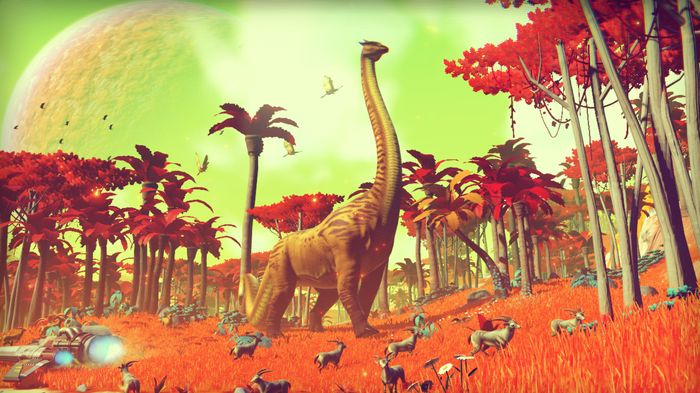
\includegraphics[width=4in]{../images/no-mans-sky.jpg}
\caption{Screenshot από το παιχνίδι No Man's Sky (2016). Οι κόσμοι που δημιουργεί είναι εξ'ολοκλήρου κατασκευασμένοι με τη χρήση ντετερμινιστικών μεθόδων Procedural Content Generation.}
\end{figure}

\section{Game Content}
Για να κατανοήσουμε καλύτερη το πεδίο του PCG πρέπει πρώτα να καταλάβουμε τι θεωρείται περιεχόμενο σε ένα παιχνίδι. Ο τομέας του PCG αναφέρεται και έχει χρησιμοποιηθεί σε ηλεκτρονικά παιχνίδια (Video Games), επιτραπέζια παιχνίδια (Board Games), παιχνίδια με κάρτες (Card Games) κ.ά. Στην συγκεκριμένη εργασία, επικεντρωθήκαμε στα Video Games.

\begin{description}
\item [Game Content] Όπως αναφέρεται και στο όνομα, περιεχόμενο, είναι κάτι που περιέχεται σε ένα παιχνίδι. Αυτός ο ορισμός όμως είναι πολύ γενικός και ευρύς και δεν περιορίζετε μόνο στο περιεχόμενο που αντιστοιχεί στο PCG. Στην βιβλιογραφία μπορούμε να ξεχωρίσουμε συγκεκριμένα είδη περιεχομένου που φαίνετε να μπορούν να δημιουργηθούν με μεθόδους PCG. Αυτά είναι:
\end{description}

\begin{itemize}
  \item Γραφικά (Textures)
  \item Επίπεδα (Levels) και χάρτες (Maps)
   \item Αντικείμενα (Items)
   \item Αποστολές (Quests)
   \item Ιστορίες (Stories)
   \item Μουσική (Music)
\end{itemize}

Ο παραπάνω διαχορισμός γίνεται με βάση το είδος του κάθε περιεχομένου, για παράδειγμα η μουσική ως περιεχόμενο ενός παιχνιδιού, διαφέρει από τα αντικείμενα. Αντίστοιχα οι μεθοδολογίες που έχουν αναπτυχθεί για την παραγωγή μουσικής διαφέρουν από τις μεθόδους που χρησιμοποιούνται για την παραγωγή αντικειμένων. Αυτό βέβαια δεν σημαίνει ότι δεν υπάρχουν κοινοί αργόριθμοι που μπορούν να εφαμροστούν σε παραπάνω από ένα είδος με επιτυχία, αντίθετα υπάρχουν πολλοί αλγόριθμοι που έχουν ως βάση έναν πιο γενικό αλγόριθμο και αποτελούν ειδικές εκδόσεις του για το κάθε είδος περιεχομένου.
\par
Ο διαχωρισμός του περιεχομένου βοηθάει στην καλύτερη κατανόηση των ιδιαιτεροτήτων και των περιορισμών που εμφανίζει το κάθε είδος το οποίο οδηγεί στην δημιουργία καλύτερων μεθόδων και αλγορίθμων.

\section{Η χρησιμότητα του PCG}
	Η πρώτη ανάγκη που παρουσιάστηκε και οδήγησε στην υιοθέτηση μεθόδων PCG αφορούσε την μείωση του αποθηκευτικού χώρου που καταλάμβανε ένα παιχνίδι. Το PCG δίνει την δυνατότητα τις δημιουργίας content μόλις παρουσιαστεί η ανάγκη να χρησιμοποιηθεί ή να παρουσιαστεί στον παίκτη, το οποίο σημαίνει ότι δεν χρειάζετε να καταλαμβάνει χώρο στην μνήμη εάν υπάρχει η δυνατότητα δημιουργίας του ακριβώς την στιγμή που χρειάζεται. Με την μνήμη να αποτελεί έναν διαμοιραζόμενο πώρο μεταξύ των εφαμρογών ακόμα και σήμερα το PCG αποτελεί μια μέθοδο μείωσης του χώρου που καταλαμβάνει ένα παιχνίδι.
\par
	Το PCG έχει επίσης χρησιμότητα από τους καλλιτέχνες και σχεδιαστές διαφόρων παιχνιδιών. Η χρήση PCG για την δημιουργία περιεχομένου το οποίο αν και δεν είναι τέλειο ή αρκετά καλό για το παιχνίδι, δίνετε στους σχεδιαστές οι οποίοι το βελτιώνουν, το αλλάζουν και προσθέτουν στοιχεία ώστε προστεθεί με επιτυχία στο παιχνίδι. Με αυτόν τον τρόπο το PCG βοηθάει τους ανθρώπους με τέτοιους ρόλους στην εργασία τους, δίνοντας του έμπνευση και κάνοντας ένα κομμάτι της δουλειάς ώστε αυτοί να μπορούν να δώσουν προσοχή στις λεπτομέρειες που θα κάνουν το περιεχόμενο πραγματατικά εντυπωσιακό. Σε αυτές τις υλοποιήσεις του PCG συνηθίζεται να δίνει ο σχεδιαστής μέσω διαφόρων εισόδων κάποιες παραμέτρους που ορίζουν μια γενική περιγραφή του περιεχομένου που θέλει να δημιουργήσει, για παράδειγμα το μέγεθος του χάρτη ή το είδος των πόρων που θα έχει διαθέσιμα. Στη συνέχεια το PCG δημιουργεί το περιεχόμενα με βάση τις παραμέτρους που πήρε και εμφανίζει το αποτέλεσμα στο σχεδιαστή. Αυτή η διαδικασία μπορεί να επαναληφθεί πολλές φορές μέχρι να δημιουργεί το επιθυμητό αποτέλεσμα.
\par
	Μια επίσης πολύ σημαντική ανάγκη που καλύπτει, εν μέρη, το PCG είναι η δημιουργία ενός παιχνιδιού που δεν τελειώνει ποτέ. Αντίθετα με την συνεχή παραγωγή πρωτότυπου και ποικίλου περιεχομένου, ένα παιχνίδι μπορεί να συνεχίζετε επ άπειρον, προσφέροντας αμέτρητες ώρες gameplay στους παίκτες. Πολλά παιχνίδια έχουν επιχειρήσει να υλοποιήσουν αυτό το feauture, κάποια με μεγάλη επιτυχία και κάποια με το αντίθετο αποτέλεσμα. Ένα από τα μεγαλύτερα προβλήματα που αντιμετωπίζουν οι υλοποιήσεις του PCG είναι η επαναληψιμότητα και η μονοτονία, όπως θα αναλυθεί και παρακάτω. Είναι ένα από τα πιο σημαντικά κριτήρια για την επιτυχία ενός endless παιχνιδιού.
\par
	Τέλος, μια ανάγκη που έχει προκύψει τα τελευταία χρόνια στον χώρο των παιχνιδιών και συνδέετε με μια ακόμα περιοχή της Τεχνητής Νοημοσύνης στα παιχνίδια είναι η εξατομίκευση περιεχομένου, ή personalized content. Αναφέρεται στην δημιουργία περιεχομένου που είναι σχεδιασμένο για τις προτιμήσεις και τις ανάγκες του κάθε παίκτη.

\section{Παιχνίδια που χρησιμοποιούν PCG}

Από την πρώτη στιγμή που ξεκίνησε η διάδωση των Video Games φάνηκε η ανάγκη για την αυτόματη και αυτόνομη δημιουργία   \textit{σωστού} περιεχομένου. Κάποια από τα παιχνίδια που εφάρμοσαν με μεγάλη επιτυχία μεθόδους PCG είναι:

\begin{description}
\item [Rogue (\textbf{1980})] Ένα από τα πρώτα παιχνίδια που εφάρμοσε PCG για την αυτόματη δημιουργία επιπέδων (\textbf{levels}). To Rogue ενέπνευσε την δημιουργία πολλών παιχνιδιών με αντίστοιχες δυνατότητες και PCG μεθόδους.

\item [Spore (\textbf{2008})] To Spore είναι ένα life-simulation και strategy παιχνίδι που χρησιμοποιεί PCG για την δημιουργία πλασμάτων και αντικειμένων. Οι αλγόριθμοι του Spore, συνδυάζουν απλά σχήματα και αντικείμενα για να δημιουργήσουν μεγαλύτερα και πιο πολύπλοκα πλάσματα με βάση διάφορους κανόνες και περιορισμούς. 

\item [No Man's Sky (\textbf{2016})] Ένα από τα πιο σημαντικά παραδείγματα για τις δυνατότητες του PCG είναι το παιχνίδι no Man's Sky. Το θέμα του παιχνιδιού είναι η εξερεύνηση του διαστήματος και η επιβίωση σε ξένους πλανήτες. Το παιχνίδι δημιουργεί σχεδόν όλόκληρο τον κόσμο με PCG, δηλαδή τους πλανήτες, τα αστέρια, τα φυτά, τα ζώα και τα encounters του παίκτη με τη χρήση ντετερμινιστικών αλγορίθμων PCG. Η αποδοχή του παιχνιδιού από το κοινό ήταν μέτρια. Οι δημιουργοί είχαν υποσχεθεί έναν απέραντο κόσμο γεμάτο περιεχόμενο και οι παίκτες παρατήρησαν ότι το τελικό αποτέλεσμα ήταν μονότονο και επαναλαμβανόμενο, κάτι που τους δημιούργησε άσχημες εντυπώσεις. 
\end{description}

\section{Προβλήματα του PCG}
Όπως αναφέρθηκε και παραπάνω, το PCG δεν αποτελεία μια τέλεια και ολοκληρωμένη λύση για να τα προβλήματα που καλείται να αντιμετωπίσει. Αντίθετα οι υλοποιήσεις του PCG πρέπει να λαμβάνουν υπόψη τα καινούργια προβλήματα και περιορισμούς που δημιουργούνται με την χρήση PCG αλγορίθμων. 

\begin{description}
\item [Επαναληψιμότητα - Μονοτονία] Ένα από τα πιο σημαντικά θέματα είναι η ποικιλία και μοναδικότητα του παραγόμενου περιεχομένου. Όπως αναλύθηκε και παραπάνω, σε πολλές περιπτώσεις το παραγόμενο περιεχόμενο είναι πολύ μονότονο, μοτίβα φαίνονται να επαναλαμβάνονται και κατά συνέπεια το αποτέλεσμα δίνει στον χρήστη την αντίθετη εντύπωση από την επιθυμητή. Οι λόγοι που συμβαίνει αυτό είναι πολλοί και σχετίζονται με το είδος του αλγόριθμου που χρησιμοποιείται κάθε φορά, τις παραμέτρους που δίνονται και τα βασικά assets που χρησιμοποιεί για να δημιουργήσει το περιεχόμενο. 

\item [Ταχύτητα - πολυπλοκότητα] Πολλοί αλγόριθμοι PCG πρέπει να είναι σε θέση να λειτουργούν σε πολύ λίγο χρόνο και με περιορισμένους πόρους. Σε ένα ηλεκτρονικό παιχνίδι υπάρχουν πολλά κομμάτια που πρέπει να δουλεύουν ταυτόχρονα, όπως τα γραφικά, το UI, το σύστημα κανόνων για την προσομοίωση της φυσικής στον κόσμο του παιχνιδιού κ.ά. Συνεπώς το σύστημα του AI που περιέχει και το PCG δεν μπορεί να καταλαμβάνει πολλούς πόρους ή να αργεί να ανταποκριθεί γιατί το παιχνίδι θα φαίνετε να κολλάει ή να μην δουλεύει όπως πρέπει. Αυτό σημαίνει ότι οι αλγόριθμοι που υλοποιούν το PCG πρέπει να έχουν συγκεκριμένη χρονική και χωρική πολύπλοκότητα και να μην ξεπερνάνε.

\item [Playability] Μπορεί να έχουμε σχεδιάσει τον τέλειο αλγόριθμο PCG που χρησιμοποιεί ελάχιστους πόρους του συστήματος και δημιουργεί μοναδικά επίπεδα για το 2D platformer παιχνίδι μας αλλά ένα στα τρία επίπεδα να μην έχουν είσοδο.Αυτό σημαίνει ότι ο παίκτης δεν θα μπορέσει να το επισκεφτεί ποτέ, ή θα βρεθεί παγιδευμένος μέσα του χωρίς κάποιο τρόπο να προχωρήσει το παιχνίδι. Αυτό φυσικά είναι κάτι που δεν θέλουμε σε καμία περίπτωση να συμβεί. Για αυτό το λόγο πρέπει να ορίσουμε τι θεωρείται "playable" περιεχόμενο και τι "unplayable".
 
\end{description}


\section{Επιθυμητά Χαρακτηριστικά του PCG}
Με βάση τα παραπάνω στοιχεία μπορούμε να αναλύσουμε ένα σύνολο από επιθυμητά χαρακτηριστικά που θέλουμε να έχει κάθε σύστημα PCG ώστε να διασφαλίσουμε την σωστή και αρμονική λειτουργία του μέσα στο παιχνίδι.

\subsection{Ταχύτητα - Πολυπλοκότητα} Όπως είδαμε και στο 1.4 ένα μεγάλο θέμα για κάθε παιχνίδι είναι η διαχείριση και κατανομή των πόρων στα επιμέρους συστήματα του. Το σύστημα του AI, που περιέχει και το υποσύστημα του PCG πρέπει να περιορίσει την πολυπλοικότητα των αλγορίθμων του, χρονικά και χωρικά, ώστε να ανταποκρίνονται στους διαθέσιμους πόρους. Αυτός ο περιορισμός είναι ιδιαίτερα σημαντικός για την επιτυχία του παιχνιδιού καθώς η εμπειρία του παίκτη σχετίζετε άμεσα με την πόσο γρήγορα και σωστά ανταποκρίνεται το παιχνίδι. 
\par
Εάν το αλγόριθμος που δημιουργεί personalized όπλα για τον παίκτη αργήσει να ολοκληρώσει την λειτουργία του, θα φανεί στον παίκτη ότι το παιχνίδι έχει "κολλήσει" και δεν ανταποκρίνεται με συνέπεια να πάρει μια αρνητική εμπειρία από το gameplay του. Αντίθετα παιχνίδια που καταφέρνουν να ανταποκρίνονται άμεσα σε κάθε εντολή του παίκτη λαμβάνουν πολύ θετικό feedback τόσο από το κοινό όσο και από κριτικούς του χώρου.

\subsection{Δημιουργικότητα - πρωτοτυπία} Το ιδανικό σύστημα PCG θα δημιουργεί περιεχόμενο αντίστοιχο με το περιεχόμενο που δημιουργεί ένας designer σε θέμα προτοτυπίας και δημιουργηκότητας. Όπως είδαμε από τα παραδείγματα παραπάνω αυτό δεν ισχύει καθολικά ή στον βαθμό που θέλουμε πάντα. Είναι πολύ δύσκολη η καταγραφή και έκφραση της δημιουργηκότητας με όρους που μπορεί να καταλάβει ένας αλγόριθμος. Αποτελεί ακόμα ένα ανοιχτό πρόβλημα στον χώρο της Τεχνητής Νοημοσύνης και επηρεάζει άμεσα τα αποτελέσματα του PCG.
\par
Παρόλαυτα έχουν γίνει πολλές προσπάθειες και βελτιώσεις σε αυτό το χαρακτηριστικό του PCG ιδιαίτερα με την χρήση βαθιών νευρωνικών δικτύων. Επίσης το παραγόμενο περιεχόμενο θέλουμε να δίνει την εντύπωση ότι δεν δημιουργήθηκε από κάποιον αλγόριθμο, αλλά από κάποιον άνθρωπο. Αυτό το χαρακτηριστικό είναι πολύ δύσκολο να επιτευχθεί. Με την αύξηση της χρήσης του PCG στα παιχνίδια, οι παίκτες "έμαθαν" να ξεχωρίζουν το περιεχόμενο που παράγετε από αλγορίθμους και να προσπαθούν σε πολλές περιπτώσεις να το χρησιμοποιήσουν προς όφελος τους για να "παρακάμψουν" κανόνες του παιχνιδιού.
\par
Για παράδειγμα στο παιχνίδι Mount and Blade II Bannerlord (2020) υπάρχει η πιθανότητα το παιχνίδι να δημιουργήσει μάχες κατά την διάρκεια αποστολών για να τις κάνει πιο δύσκολες και ενδιαφέρον. Οι παίκτες γνωρίζοντας ότι το σύστημα του PCG υπολογίζει την πιθανότητα μάχης εκείνη την στιγμή, μπορούν να φορτώσουν το παιχνίδι σε κάποια προηγούμενη στιγμή και όταν φτάσουν στο σημείο της μάχης, το σύστημα να ξανα υπολογίσει την πιθανότητα, αυτή την φορά βγάζοντας αρνητική πιθανότητα μάχης. 

\subsection{Aξιοπιστία} H αξιοπιστία του παραγόμενου περιεχομένου συνδέετε άμεσα με μια πολύ απλή ερώτηση: Είναι playable? Μπορεί δηλαδή το περιεχόμενο που παράχθηκε να προστεθεί στο παιχνίδι και να το χρησιμοποιήσει ο παίκτης όπως πρέπει ή δημιουργεί προβλήματα, για παράδειγμα ένα laser gun χωρίς σκανδάλη ή χωρίς την λειτουργικότητα της σκανδάλης είναι άχρηστο. Εκτός από το αν είναι χρήσιμο, το περιεχόμενο θα πρέπει να μην "σπάει" το παιχνίδι. Δηλαδή να μην παγιδεύει το παίκτη σε καταστάσεις από τις οποίες δεν μπορεί να συνεχίσει την πρόοδο του ή να του δίνει πλεονεκτήματα που σπάνε τους κανόνες του παιχνιδιού.
\par
Για τον έλεγχο της αξιοπιστίας του παραγόμενου περιεχομένου υπάρχουν οι Evaluators, οι οποίοι είναι αλγόριθμοι του συστήματος PCG και "αποφασίζουν" εάν το περιεχόμενο που παράχθηκε είναι playable ή όχι. Εάν το αξιολογίσουν ως unplayable, ο PCG αλγόριθμος πρέπει να δημιουργήσει ένα καινούργιο μέχρι να περάσει την αξιολόγηση ακιοπιστίας.

\subsection{Παραμετροποιησιμότητα} Σε όλους τους αλγόριθμους PCG δίνονται κάποιοι παράμετροι ως είσοδος. Από αυτές τις παράμετρους εξαρτώνται συγκεκριμένα χαρακτηριστικά που θα έχει το παραγόμενο αποτέλεσμα. Αυτό το χαρακτηριστικό είναι πολύ σημαντικό για τα συστήματα PCG που χτίζονται ως βοηθητικά συστήματα για τους designers του παιχνιδιού. Επίσης καθορίζουν πόσο ντετερμινιστικό είναι το σύστημα PCG.
\par
Για παράδειγμα το παιχνίδι Oxygen Not Included (2019), ένα παιχνίδι προσομοίωσης και επιβίωσης, δημιουργεί το επίπεδο στο οποίο ο παίκτης θα πρέπει να χτίσει την βάση του, παίρνοντας ως είσοδο ένα hash. Αυτό το hash μπορεί να παραχθεί τυχαία από το παιχνίδι ή να το δώσει ο παίκτης, με αποτέλεσμα παίκτες να μπορούν να βρουν και να ανταλλάξουν hash για επίπεδα που τους φάνηκαν πολύ ευνοικά ή πολύ δύσκολα. Το συγκεκριμένο χαρακτηριστικό φάνηκε να βελτιώνει την εμπειρία των παικτών με το παιχνίδι καθώς δημιουργήθηκε ένα community που μοιραζόταν hash από επίπεδα και σύγκριναν τις εμπειρίες και τα score τους.

% leave 60mm empty space below
\vspace{60mm}

\section{Procedural Content Generation για 2D επίπεδα}

Ένας τομέας με εκτενείς εφαρμογές του PCG είναι τα 2D παιχνίδια και η δημιουργία επιπέδο (levels) ή dungeon για αυτά. Ένα τέτοιο επίπεδο μπορεί να οριστεί ως ένας 2D χώρος, ο οποίος περιέχει δωμάτια ή χώρους, χωρισμένα με διαχωριστικά ή άλλα εμπόδια. Ο παίκτης μπορεί να περιηγηθεί στο επίπεδο με βάση τους κανόνες του κάθε παιχνιδιού, είτε μέσα από πόρτες και ανοίγματα ή ανοίγοντας τρύπες στα διαχωριστικά. Καθώς εξερευνεί μπορεί να συναντήσει αντικείμενα, τέρατα, κρυφά περάσματα κ.ά. 
\par
Σε αυτή την εργασία αναπτύχθηκαν αλγόριθμοι και μοντέλα για την δημιουργία τέτοιων επιπέδων οπότε είναι σημαντικό να αναλυθούν οι διάφοροι περιορισμοί και ιδιαιτερότητες αυτού του τομέα, καθώς και άλλες γνωστές μέθοδοι και τα χαρακτηριστικά τους.
\par
Η μελέτη και επιλογή αυτού του τομέα είναι ιδιαίτερα διαδεδομένη στην επιστημονική κοινότητα του PCG καθώς προσφέρει μια ένα χώρο αναζήτησης που μπορεί εύκολα να αναπαρασταθεί και να αποθηκευτεί σε διάφορες μορφές. Επίσης είναι εύκολο το evaluating και το testing τέτοιου περιεχομένου όπως θα αναλυθεί και παρακάτω.

\subsection{Εισαγωγή}
Όπως περιγράφετε και στο Procedural Content Generation in Games, το PCG για την δημιουργία τέτοιων επιπέδων περιέχει την δημιουργία της τοπολογίας, της γεωμετρίας και των αντικειμένων του επιπέδου. Επίσης το παραπάνω βιβλίο αναλύει την διαδικασία του PCG για επίπεδα σε τρία βασικά στοιχεία:

\begin{description}
  \item[$\bullet$ Μοντέλο αναπαράστασης] Αποτελεί μια απλοποιημένη και γενική αναπαράσταση ενός επιπέδου.
  \item[$\bullet$ Μέθοδο δημιουργίας του μοντέλου αναπαράστασης] Αποτελεί τον αλγόριθμο που δημιουργεί καινούργια επίπεδα ως το μοντέλο αναπαράστασης που έχει οριστεί για αυτά. 
    \item[$\bullet$ Μέθοδο δημιουργίας του επιπέδου από το μοντέλο αναπαράστασης] Αυτή η μέθοδος αναλαμβάνει να δημιουργήσει το επίπεδο στον χώρο του παιχνιδιού με βάση το μοντέλο αναπαράστασης που δημιούργησε η μέθοδος δημιουργίας. Αυτό είναι το αποτέλεσμα που θα δει ο χρήστης.
\end{description}

Θα αναλυθούν μερικές οικογένειες αλγορίθμων PCG για 2D επίπεδα. Αυτές είναι οι πιο γνωστοί και ευρέως χρησιμοποιούμενοι αγλόριθμοι για αυτόν τον τομέα του PCG. Με μια σύντομη περιγραφή είναι:

\begin{description}
  \item[$\bullet$ Διαχωρισμός χώρου (Space Partitioning)] 
  \item[$\bullet$ Με την χρήση πρακτόρων (Agent-based)]
    \item[$\bullet$ Cellular Automata] 
    \item[$\bullet$ Με τη χρήση γραμματικών (Generative Grammars)] 
\end{description}

\subsection{Space Partitioning}
Αυτή η ομάδα αλγορίθμων χρησιμοποιείται και σε άλλες περιοχές του game development όπως τα γραφικά, οπότε οι μεθοδολογίες και οι δομές δεδομένων είναι γνωστά στους σχεδιαστές και προγραμματιστές παιχνιδιών. Όπως περιγράφει και το όνομα της, εκτελεί έναν διαχωρισμό του χώρου σε υποχώρους. Αυτό μπορεί να χρησιμοποιηθεί στο PCG για την δημιουργία δωματίων και διαδρόμων μέσα σε ένα  συγκεκριμένο χώρο.
\par
Ένας αλγόριθμος που χρησιμοποιείται πολύ σε υλοποιήσεις space partitioning (BSP) είναι ο binary space partitioning και παραλλαγές του όπως quadtree space partitioning και octree space partitioning. Θα αναλύσουμε τον βασικό αλγόριθμο του BSP, περιγραφές για τους quadree και octree μπορούν να βρεθούν εδώ.

\begin{description}
  \item[$\bullet$ Binary Space Partitioning (BSP)]
  Ο αλγόριθμος είναι αναδρομικός και χτίζει το επίπεδο ιεραρχικά χρησιμοποιώντας ως δομή δεδομένων ένα binary tree. Στο root node του tree περιέχεται "ολόκληρο" επίπεδο. Στην πρώτη αναδρομή, το επιλεγμένο node, το root σε αυτή την περίπτωση χωρίζεται σε δύο τμήματα με κάποιον ορισμένο διαχωρισμό, για παράδειγμα κάθετα. Αυτά τα δύο κομμάτια προστίθονται ως child nodes στο root και στη συνέχεια ο αλγόριθμος καλείται για κάθε ένα από τα παιδιά.
  \par
  Ο αλγόριθμος σταματάει όταν φτάσει σε κάποια ορισμένη τερματική συνθήκη, για παράδειγμα βάθος δέντρου n ή μόλις τελειώσουν τα nodes που υπάρχουν για να partitioning. Για να προστεθεί τυχαιότητα στον αλγόριθμο, άρα κατα συνέπεια και διαφορροποίηση στα παραγόμενα επίπεδα σε κάθε εκτέλεση, μπορεί να αποδοθεί μια πιθανότητα διαχωρισμού σε κάθε node. Εαν η πιθανότητα είναι κάτω από ένα κατώφλι να μην γίνετε διαχωρισμός αυτού του επιπέδου. Επιπλέον το κατώφλι μπορεί να διαμορφώνετε ανάλογα με το μέγεθος του παραγώμενου επιπέδου ή το βάθος που βρίσκεται αυτή τη στιγμή ο αλγόριθμος.
  \par 
  Η εισαγωγή και δοκιμή τέτοιων παραμέτρων είναι ένα μεγάλο κομμάτι της υλοποίησης, και παίζει καθοριστικό ρόλο στο τελικό αποτέλεσμα. Επίσης τέτοιου είδους παράμετροι μπορούν να χρησιμοποιηθούν από τους σχεδιαστές για να παράγουν διαφόρων ειδών επίπεδα.
\end{description}

